% System diagram for the Assignment 2 report. Build: pdflatex architecture.tex -> architecture.pdf
% Style follows the group's other papers: Times (mathptmx), thin rounded boxes, light fills by stage type.
\documentclass[border=2pt]{standalone}
\usepackage{mathptmx}
\usepackage{amsmath,amssymb}
\usepackage{tikz}
\usetikzlibrary{arrows.meta,positioning,fit,calc,backgrounds}
\DeclareMathOperator{\CE}{CE}
\DeclareMathOperator{\JS}{JS}
\DeclareMathOperator{\Rev}{Rev}
\begin{document}
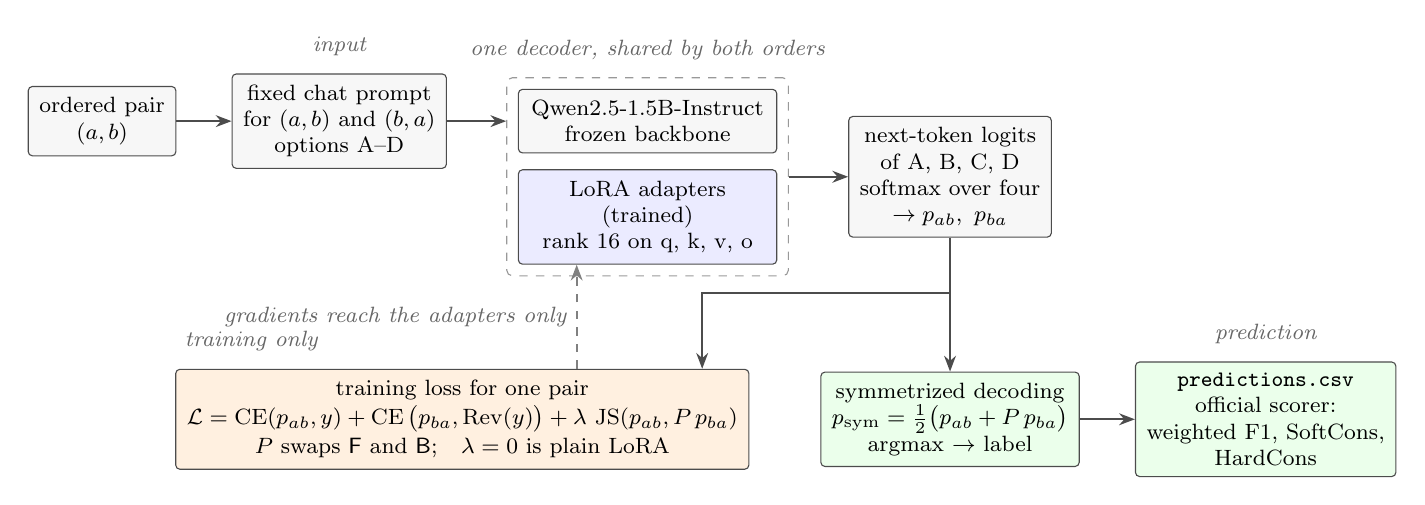
\begin{tikzpicture}[
  font=\footnotesize,
  box/.style={draw=black!70, rounded corners=1.5pt, align=center,
              inner sep=4pt, minimum height=6.5mm, fill=black!3},
  lora/.style={draw=black!70, rounded corners=1.5pt, align=center,
               inner sep=4pt, minimum height=6.5mm, fill=blue!8},
  train/.style={draw=black!70, rounded corners=1.5pt, align=center,
                inner sep=4pt, minimum height=6.5mm, fill=orange!12},
  pred/.style={draw=black!70, rounded corners=1.5pt, align=center,
               inner sep=4pt, minimum height=6.5mm, fill=green!8},
  group/.style={draw=black!40, dashed, rounded corners=2pt, inner sep=4pt},
  arr/.style={-{Stealth[length=2mm]}, black!70, thick},
  back/.style={-{Stealth[length=2mm]}, black!50, thick, dashed},
  lbl/.style={font=\footnotesize\itshape, black!60}
]
% ---------------- shared forward pass (top) ----------------
\node[box] (in) {ordered pair\\$(a,b)$};
\node[box, right=7mm of in] (prompt) {fixed chat prompt\\for $(a,b)$ and $(b,a)$\\options A--D};
\node[box, right=9mm of prompt, text width=30mm] (bb) {Qwen2.5-1.5B-Instruct\\frozen backbone};
\node[lora, below=2mm of bb, text width=30mm] (lora) {LoRA adapters (trained)\\rank 16 on q, k, v, o};
\begin{scope}[on background layer]
  \node[group, fit=(bb)(lora)] (dec) {};
\end{scope}
\node[box, right=9mm of bb.east |- dec.east, anchor=west] (score) {next-token logits\\of A, B, C, D\\softmax over four\\$\rightarrow p_{ab},\ p_{ba}$};
\draw[arr] (in) -- (prompt);
\draw[arr] (prompt.east) -- (prompt.east -| dec.west);
\draw[arr] (dec.east |- score.west) -- (score.west);
\node[lbl, above=1mm of dec.north] {one decoder, shared by both orders};
\node[lbl, above=1mm of prompt.north] {input};

% ---------------- prediction branch (bottom right) ----------------
\node[pred, below=17mm of score] (sym) {symmetrized decoding\\$p_{\mathrm{sym}}=\tfrac12\big(p_{ab}+P\,p_{ba}\big)$\\argmax $\rightarrow$ label};
\node[pred, right=7mm of sym] (scorer) {\texttt{predictions.csv}\\official scorer:\\weighted F1, SoftCons,\\HardCons};
\draw[arr] (sym) -- (scorer);
\node[lbl, above=1mm of scorer.north] {prediction};

% ---------------- training branch (bottom left) ----------------
\node[train, left=9mm of sym] (loss)
  {training loss for one pair\\[1pt]
   $\mathcal{L}=\CE(p_{ab},y)+\CE\big(p_{ba},\Rev(y)\big)+\lambda\,\JS(p_{ab},P\,p_{ba})$\\[1pt]
   $P$ swaps \textsf{F} and \textsf{B};\quad $\lambda=0$ is plain LoRA};
\node[lbl, above=1mm of loss.north west, anchor=south west] {training only};

% ---------------- connections between the rows ----------------
\coordinate (j) at ($(score.south)+(0,-7mm)$);
\draw[black!70, thick] (score.south) -- (j);
\draw[arr] (j) -| (sym.north);
\draw[arr] (j) -| ($(loss.north east)+(-6mm,0)$);
\coordinate (g) at ($(lora.south)+(-9mm,0)$);
\draw[back] (g |- loss.north) -- node[lbl, left] {gradients reach the adapters only} (g);
\end{tikzpicture}
\end{document}
